\documentclass{article}
\usepackage[top=1in, bottom=1in, left=1in, right=1in]{geometry}
\usepackage{fancyvrb}
\usepackage{multirow}
\usepackage{graphicx}
\usepackage{enumerate}
\DefineShortVerb{\|}
\pagenumbering{gobble}

\usepackage{titlesec}
\titleformat{\section}[block] {\normalfont\bfseries\Large}{\fbox{\thesection}}{1em}{}
\titlespacing{\section}{0pt}{*6}{*1}
\titleformat{\subsection}[block] {\normalfont\bfseries\large}{\thesubsection}{1em}{}


\begin{document}

\title{SISMID Module 9\\Lab 5: Intervention strategies}
\author{Thomas J. Hladish, Shweta Bansal, Joel C. Miller and Lauren Ancel Meyers}
\date{July 2015}
\maketitle


\section*{Implementing intervention strategies}

In this course, we have talked about a number of different intervention strategies. We can model some of these 
strategies using the percolation simulation that we developed in the last lab.  In this case, we will use
the Vancouver urban network that we used previously in Lab~1 (|urban_net.csv|).  Let's look at the effects of
three intervention strategies in particular: two vaccination strategies and one ``social distancing'' strategy.

Since vaccination makes it impossible for an individual to get infected (assuming a 100\% effective vaccine), we can
model vaccination by removing nodes from the network, or more generally by making it impossible for those nodes to participate in the epidemic.

Since ``social distancing'' reduces an individual's disease-causing contacts, we can model this strategy by
removing edges from the network.

I've given you a head start with a fairly fast implementation of the percolation simulation.  You can download the program 
from the link ``Lab 4: Intervention percolation code.''  (This code is also reproduced in the appendix to this lab.)  Run the program as-is,
and record the mean epidemic size when no intervention measures are in place.  Call it S.

Now implement the following strategies:
\begin{enumerate}
\item Locate the commented block with the words ``Implement intervention strategy here'' (Line~40).  Write a block 
of code that vaccinates 17.8\% of the population \textbf{randomly}. Hint: the easiest way to do this is to loop through
all nodes, and with 17.8\% probability delete all of that node's edges.  Now run the program and record the mean epidemic size. Call it S1.
\item For each individual vaccinated, how many people did the random vaccination strategy prevent from
becoming sick? That is, to what extent did we achieve herd immunity?
\item Write intervention code that vaccinates the 17.8\% of the population with the highest degrees.  Hint: 17.8\% of the urban
network is 480 nodes.  If you vaccinate all individuals with degree greater than or equal to 23, you will vaccinate the top 17.8\%.  Run the
simulation again, and call the resulting mean epidemic size S2.
\item Write intervention code that \textbf{randomly} reduces each individual's edges by 17.8\%.
Run the percolation simulation again, and record the resulting epidemic size.  We'll call this S3.
\item Compare the four epidemic sizes (S, S1, S2, S3).  How much of a reduction in epidemic size
 did each control strategy yield, relative to S?  Which strategy is best?
\item Which of these strategies do you think would be easiest to implement
practically/logistically/ethically? How does one implement the second strategy in practice? (i.e.
How do we know who in the population is ``high degree''?)

\end{enumerate}
\section*{Additional exercise: Age-based strategies}
Download the urban network ages file, |urban_ages.csv|.  Take a
moment to look at the contents of the ages file: notice that it is structured
much like an edge list file, but in this case only the first column contains node
names (which are integers), while the second column contains age classes.  These
classes are as follows:

\UndefineShortVerb{\|}
\begin{figure}[h]
\begin{center}
% use packages: array
\begin{tabular}{|ll|}
\hline
Age class & Description \\ \hline
1 & Infants and toddlers (age $<$ 3) \\ 
2 & Preschoolers (3 $\leq$ age $<$ 5) \\ 
3 & Children (5 $\leq$ age $<$ 18) \\ 
4 & Adults (18 $\leq$ age $<$ 50) \\ 
5 & Elderly living at home (50 $\leq$ age) \\ 
6 & Nursing home residents (65 $\leq$ age) \\
\hline
\end{tabular}
\caption{Age class definitions for Vancouver urban network}
\end{center}
\end{figure}
\DefineShortVerb{\|}

Ages are also strongly characterized by different mean degrees:
\begin{figure}[h]
\begin{center}
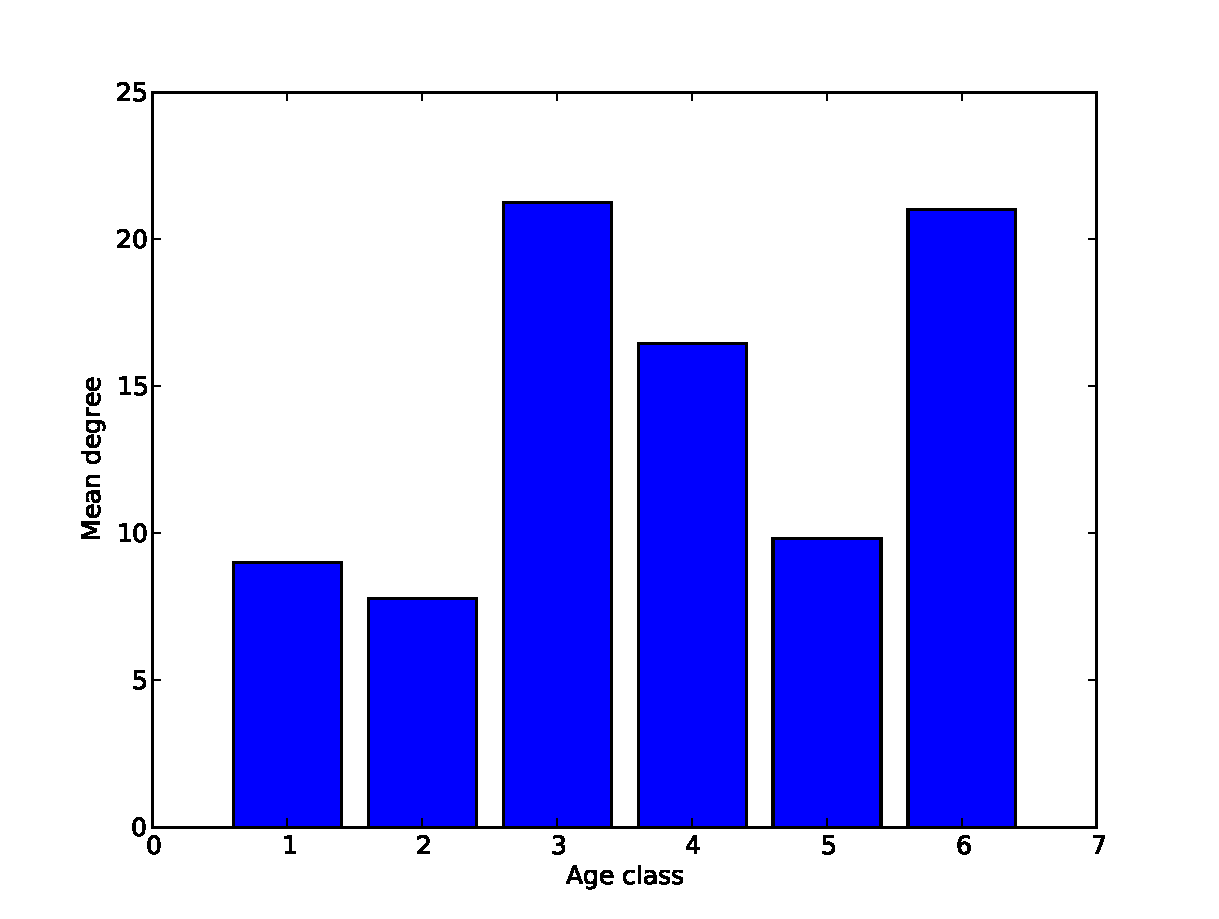
\includegraphics[width = 5in]{age_vs_deg.pdf}
\caption{Age versus mean degree for Vancouver urban network}
\end{center}
\end{figure}

Try implementing the following vaccination strategies:
\begin{itemize}
\item As suggested in the previous exercise, identifying high-degree people directly may be difficult.  If we know,
however, that age can be an indicator of degree, how might we design and implement a vaccination strategy to target high-degree individuals?
Does the effectiveness of this approach warrant its use?
\item Now consider that for influenza, the very young and the very old are the most likely to die due to primary or secondary infection.  How should we
weight preventing death versus preventing illness?  Do we prevent more death by vaccinating the vulnerable, or by vaccinating the high-degree individuals?
\end{itemize}



\pagebreak
\section*{Appendix: \texttt{intervention\_perc.py}}
You may download this file, but sometimes seeing a printed copy makes reading code easier.
\begin{Verbatim}[numbers=left, samepage=true]
#!/usr/bin/python                                                                                         
from networkx import *                                                                                    
from random import *                                                                                      
from pylab import mean                                                                                    

### Define percolation simulation, using graph G and transmissibility T
def percolate(G, T):                                                   
    states = dict([(node, 's') for node in G.nodes()])                 

    p_zero = choice(G.nodes())
    states[p_zero] = 'i'      
    infected = [p_zero]       
    recovered = []

    while len(infected) > 0:
        v = infected.pop(0)
        for u in G.neighbors(v):
            if states[u] == 's' and random() < T:
                states[u] = 'i'
                infected.append(u)
        states[v] = 'r'
        recovered.append(v)
    ### return the epi size as a fraction of the ORIGINAL population
    return len(recovered)/float(net_size)

### Set transmissibility
### Corresponds to an R0 of about 2.5 for the urban network
T = 0.1357

### Build urban network
file = open("urban_edges.csv")
G = Graph()
for edge in file:
    node1, node2 = edge.strip().split(',')
    G.add_edge(node1, node2)
net_size = G.order()


############################################
### Implement intervention strategy here ###
############################################


### Run the simulation a bunch of times
results = []
for i in range(100):
    s =  percolate(G, T)
    results.append(s)

### Print the mean epidemic size
print mean(results)
\end{Verbatim}

\end{document}
